\documentclass{article}




% Language setting
% Replace `english' with e.g. `spanish' to change the document language
\usepackage[english]{babel}

% Set page size and margins
% Replace `letterpaper' with `a4paper' for UK/EU standard size
\usepackage[letterpaper,top=2cm,bottom=2cm,left=3cm,right=3cm,marginparwidth=1.75cm]{geometry}

% Useful packages
\usepackage{amsmath}
\usepackage{graphicx}
\usepackage[colorlinks=true, allcolors=blue]{hyperref}

\usepackage{tikz}


\title{The impact of AI on education}
\author{MALLET Samuel}

\begin{document}
\maketitle

\begin{abstract}
    The goal of this report is to provide a comprehensive
    overview of the impact of artificial intelligence (AI)
    on education, exploring the benefits, challenges, and
    future implications of integrating AI technologies into
    learning and teaching processes. The report aims to cover
    various aspects, from personalized learning and
    accessibility to the evolving roles of teachers and the
    development of creativity and critical thinking skills
    in the AI era.
\end{abstract}

\newpage

\tableofcontents

\section{Introduction}

\section{The Building Blocks of AI in Education: Language, Speech, and Conversation}
\subsection{Defining Artificial Intelligence}

\subsubsection{Challenges of defining AI}


Artificial Intelligence (AI) has become a buzzword in recent years, with its
applications spanning across various domains, including education. However,
defining AI is not a straightforward task due to several challenges. Firstly,
there is a lack of a universally accepted definition of AI across different
fields and contexts(https://www.semanticscholar.org/paper/6f18cf33eb6e22b1fd665bd24ddf1e9c0509a420)(https://www.semanticscholar.org/paper/147fde8bd3c092aeb9372c85cedb460d9f22a2ee).
The concept of AI is complex and multifaceted, making it challenging to arrive
at a precise, all-encompassing definition. Secondly, the rapidly evolving
nature of AI technologies makes it difficult to establish a fixed
definition(https://www.semanticscholar.org/paper/6624236a5ab39d57d2463fca646e15973a5a6a55)
(https://www.semanticscholar.org/paper/147fde8bd3c092aeb9372c85cedb460d9f22a2ee).
As AI capabilities expand, any definition may quickly become outdated.
% TODO : Similarly, when Apple's Siri virtual assistant was first introduced in 2011, it was seen as a groundbreaking AI technology. But today with the advancements of technologies such as chatgpt, it is seen as outdated. 
For instance, a simple linear regression, which is a statistical method used
to model the relationship between a dependent variable and one or more
independent variables, would be considered as AI by some, while others
would argue that it is just statistics. However, one could argue that all
artificial intelligence techniques are essentially based on statistics.
Even the latest revolutionary AIs work by "predicting the next word" based
on patterns in large datasets. Lastly, various fields, such as computer
science, philosophy, and law, approach AI from different perspectives and
with different goals in mind, leading to a range of definitions that may
not always align(https://www.semanticscholar.org/paper/d45e5a95b3442afd3028e87edd060fcbacd128dc)
(https://www.semanticscholar.org/paper/b1c7a9ef833287615fae3324eae044fc76839460).

\subsubsection{Common definitions}

Despite the challenges in defining AI, there are some common definitions
that are widely used. For example, Wikipedia defines AI as "intelligence
demonstrated by machines", as opposed to the natural intelligence displayed
by animals including humans. Similarly, the Oxford English Dictionary
defines AI as "The capacity of computers or other machines to exhibit or
simulate intelligent behaviour." However, these definitions are themselves
based on the concept of intelligence, which is also not a trivial task to
define.

Interestingly, what is hard for humans is often easy for computers, and vice
versa. For instance, it is hard for us to make complex computations quickly,
but simple for computers. On the other hand, it is trivial for us to recognize
animals, stop signs, talk, and drive, but these tasks are incredibly
challenging for computers to perform accurately and consistently. In practice,
what is considered as artificial intelligence is often what has been
challenging or seen as impossible for computers in the past. As computers
become more capable of performing tasks that were once thought to be the
exclusive domain of human intelligence, the definition of AI continues
to evolve and expand.

\subsection{Fields of AI}

% add the images/AI_ML_DL.png
\begin{figure} %TODO : mention this  in text
    \centering
    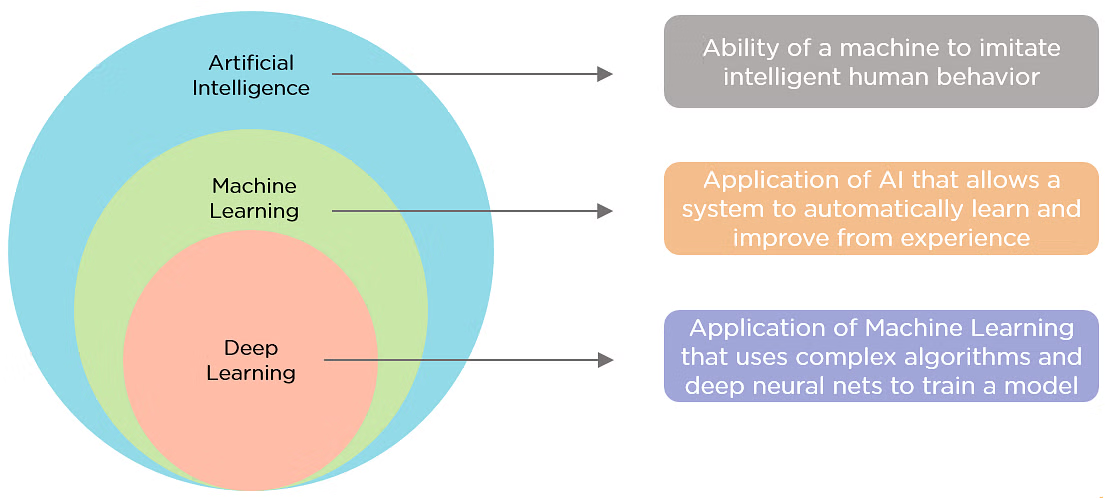
\includegraphics[width=0.8\textwidth]{images/AI_ML_DL.png}
    \caption{AI vs Machine Learning vs Deep Learning}
    %TODO : include source (https://www.simplilearn.com/tutorials/artificial-intelligence-tutorial/ai-vs-machine-learning-vs-deep-learning)
\end{figure}



The Artificial Intelligence landscape is vast and encompasses a wide range
of subfields and techniques. Nearly all the recent breakthroughs in AI
can be attributed to the subfield called Machine Learning.

\subsubsection{Introduction of Machine learning (ML)}

Machine Learning (ML) is a special type of AI programming that allows
computers to learn from data, rather than being explicitly programmed
with rules. To illustrate this concept, let's consider the task of
distinguishing between pictures of cats and dogs. It would be incredibly
difficult, if not impossible, to write down all the rules that would
account for all the possible variations in size, color, shape, and
behavior.

This is where Machine Learning comes in. Instead of trying to write down
all these rules, we can provide the computer with a large collection of
labeled pictures (i.e., pictures that have been identified as either a cat
or a dog). The computer then uses statistical techniques to find patterns
and relationships within these pictures. For example, it might learn that
dogs usually have longer noses than cats, or that cats have pointy ears
while dogs' ears are more rounded.

Once the computer has learned these patterns, it can then use them
to correctly identify cats and dogs in new pictures that it hasn't
seen before. In essence, Machine Learning is like giving the computer
a set of examples to learn from, rather than a set of rules to follow.
This makes it a powerful tool for solving complex problems that would
be too difficult for traditional programming. And the best part is,
the more data the computer has to learn from, the better it becomes
at making accurate predictions.

Machine Learning has a wide range of applications across various
domains, including image and speech recognition, natural language
processing (NLP), recommendation systems, fraud detection, predictive
maintenance, autonomous vehicles, healthcare, and many more.

\subsubsection{Deep Learning}

Nearly all the recent breakthroughs in Machine Learning can be attributed
to the field of Deep Learning. Deep Learning uses layers of artificial
"neurons" in a way that is similar to how the human brain learns.
This approach is very flexible but requires a lot of data and computer
power.

Thanks to Deep Learning, computers are now able to perform tasks that
were previously thought to be too difficult for them, such as recognizing
speech or understanding natural language. Deep Learning has revolutionized
the field of AI and has opened up new possibilities for solving complex
problems.

\subsection{The technologies we will focus on in this report}

We will not focus on AIs able to distinguish between cats and dogs, or systems that predict the price of Bitcoin. Instead, we will focus on AI technologies that can "understand" and produce human language, and allow engaging conversations between computers and humans.

\subsubsection{Natural Language Processing (NLP)}

Natural Language Processing (NLP) is an interdisciplinary subfield
of computer science and information retrieval concerned with giving
computers the ability to understand, interpret, and manipulate human
language . The goal is a computer capable of "understanding"
the contents of documents, including the contextual nuances of the
language within them.

Up until the 1980s, most NLP systems were based on complex sets of
hand-written rules. In the late 1980s, there was a revolution in NLP with
the introduction of machine learning algorithms for language processing,
due to increasing computational power. In the 2010s, representation learning
and deep neural network-style machine learning methods became widespread in
NLP, due to their achieving state-of-the-art results in many natural language
tasks.

The development of large pre-trained language models using neural networks and
vast amounts of text data has led to significant advancements in
NLP capabilities in recent years.


The development of large pre-trained language models using neural networks and vast amounts of text data has led to significant advancements in NLP capabilities in recent years.

\subsubsection{Large Language Models (LLM)}

Large Language Models (LLMs) are deep learning models trained on massive
amounts of text data to understand and generate human language. They can
perform a wide range of NLP tasks without requiring task-specific training data.
There are a large number of LLMs available, both open-source and closed-source.
Open-source models like Llama (developed by Meta), the "Mistral" models
developed by the French company Mistral, and many more are available to
researchers, companies, and the community. Closed-source models are
developed by companies like OpenAI (GPT-3, GPT-4), Anthropic (Claude),
and Google (Gemini).
LLMs range in size from millions to hundreds of billions of parameters.
Larger models generally have better performance but require more computational
resources. State-of-the-art LLMs exhibit impressive language understanding
and generation capabilities across many benchmarks and real-world
applications. However, LLMs have a limited context window, typically
a few pages of text, limiting their ability to process very long documents
or maintain long-term memory.
LLMs have various applications, such as chatbots and conversational AI
(like ChatGPT) that engage in open-ended dialogue, text generation,
summarization, translation, creative writing assistance, knowledge
retrieval, and question answering from large knowledge bases.
However, LLMs have some limitations in the education context. Training
and running large LLMs is hugely energy-intensive, raising environmental
concerns. Smaller models are more efficient and can even run on phones.
LLMs excel at pattern matching and information retrieval but struggle
with tasks requiring logical reasoning, causal understanding, and domain
expertise. They can also generate plausible but factually incorrect
statements (known as "hallucinations"), which is problematic for
educational applications where accuracy is critical.

\subsubsection{Vision}

More and more LLMs come with vision capabilities, allowing them to handle not just text but also images and even videos. LLMs can perform general-purpose vision tasks such as answering questions about image content, recognizing objects, scenes, and visual concepts, generating detailed, contextual captions and descriptions for images, visual grounding and reasoning (e.g., locating objects mentioned in a query), providing visual explanations and differentiating between similar images/classes, and enabling open-ended visual task instructions via natural language.

Some examples of vision-capable models include GPT-4 (OpenAI), the Claude 3 family of models (Anthropic), and Grok 1.5 Vision (xAI).

\subsubsection{Speech Recognition and Synthesis}

Speech recognition involves converting spoken language into written text. Previous models were not well-suited for human conversation, requiring exaggerated voice clarity and only recognizing one language at a time. Whisper, an open-source speech recognition model by OpenAI, significantly improved performance, understanding technical vocabulary and multiple languages in one conversation.

Speech synthesis has also advanced, with new models capable of simulating emotions and allowing interruptions, enabling more natural human-like conversations.

Combining speech recognition, NLP, and speech synthesis enables real-life conversations with AI, which are faster and more engaging than typing. Example applications include PI.ai, which helps users better understand their emotions without simulating affection, reducing the risk of emotional dependence (although the AI may sometimes be overly supportive), and ChatGPT voice, which allows fluid conversations, such as practicing job interviews with the AI simulating an employer role.

However, the current process of converting voice to text, processing, and converting back to voice removes emotional nuances like irony, humor, and doubt. State-of-the-art solutions are being developed to address this issue.

\subsubsection{Building on LLMs} %TODO : add examples, and clarify the RAG

Beyond chatbots in web browsers, LLMs can be integrated into a wide range of tasks. LLMs are steerable and can act as teachers, experts, or take on various roles. They enable automation and integration with other systems and workflows. For instance, LLMs can be integrated into customer service, and other examples are yet to be explored.

Retrieval-Augmented Generation (RAG) combines LLMs with external knowledge retrieval to enhance their factual accuracy and knowledge coverage.

\subsection{The Growing Influence of AI in Education}

\subsubsection{Rapid adoption of AI tools by students}
Students are increasingly using AI tools like language models and writing assistants to support their learning and complete assignments. This trend highlights the need for educators to adapt their teaching methods and assessment strategies to account for the presence of AI.

\subsubsection{Integration of AI solutions by learning platforms}
Learning management systems and educational platforms are integrating AI solutions to offer personalized learning experiences, automate grading, and provide intelligent feedback to students. This integration enables more efficient and effective learning processes.

\subsubsection{Government initiatives and policies}
Governments around the world are recognizing the potential of AI in education and implementing initiatives and policies to support its adoption. These efforts include funding research, developing guidelines for responsible AI use, and promoting digital literacy among students and educators.

\section{Benefits of AI in education}

\subsection{Personalized learning}
AI enables personalized learning experiences by adapting content, pacing, and feedback to individual student needs and preferences. This approach can lead to improved learning outcomes and increased student engagement.

\subsection{Increased accessibility to knowledge and education}
AI technologies can make education more accessible by providing intelligent tutoring systems, automated translation of learning materials, and voice-based interaction for students with disabilities. This increased accessibility can help bridge educational gaps and promote lifelong learning.

\subsection{Student engagement and motivation}
AI-powered learning tools can create interactive and engaging learning experiences that motivate students to actively participate in their education. Gamification, adaptive challenges, and immediate feedback can enhance student motivation and retention.

\subsection{Administrative efficiency and teacher support}
AI can automate administrative tasks, such as grading and record-keeping, freeing up teachers' time to focus on more high-value activities like lesson planning and student mentoring. AI-powered tools can also provide teachers with insights into student performance and learning patterns, enabling data-driven decision-making.

\section{Challenges and limitations of AI in education}

\subsection{Ensuring AI Serves as an assistant, not a substitute}
It is crucial to ensure that AI is used as an assistive tool to enhance teaching and learning, rather than a substitute for human educators. AI should complement and support the role of teachers, not replace them entirely.

\subsection{Risks of over-reliance on AI for learning}
Over-reliance on AI tools for learning can lead to students developing a shallow understanding of concepts and lacking critical thinking skills. It is essential to strike a balance between AI-assisted learning and traditional teaching methods that foster deep learning and problem-solving abilities.

\subsection{Inequalities in access to AI technologies}
The adoption of AI in education may exacerbate existing inequalities, as not all students and schools have equal access to the necessary technology and infrastructure. Efforts must be made to ensure equitable access to AI tools and resources to prevent widening educational gaps.

\section{Evolving roles of teachers and assessment methods}

\subsection{Adapting courses and exams to the AI era}
With the increasing presence of AI in education, teachers need to adapt their courses and assessment methods to account for the capabilities of AI tools. This may involve designing assignments that require higher-order thinking skills and creativity, which are less easily replicated by AI.

\subsection{AI as a complementary tool for teachers}
AI should be viewed as a complementary tool that can assist teachers in their roles, rather than a threat to their jobs. Teachers can leverage AI to personalize instruction, provide targeted feedback, and identify areas where students need additional support.

\subsection{Importance of teacher training and professional development}
To effectively integrate AI in education, it is crucial to provide teachers with adequate training and professional development opportunities. This will enable them to understand the capabilities and limitations of AI, and to effectively use AI tools to enhance their teaching practices.

\section{Future perspectives}

\subsection{Developing creativity and critical thinking in the AI era}
As AI becomes more prevalent in education, it is essential to focus on developing students' creativity and critical thinking skills. These skills will be crucial in a future where many tasks can be automated by AI, and where the ability to innovate and solve complex problems will be highly valued.

\subsection{AI and lifelong learning}
AI has the potential to support lifelong learning by providing personalized learning experiences that adapt to an individual's changing needs and interests over time. This can enable continuous skill development and help people stay relevant in a rapidly evolving job market.

\subsection{Potential for AI to bridge educational gaps in developing countries and underserved communities}
AI-powered education tools can help bridge educational gaps in developing countries and underserved communities by providing access to high-quality learning resources and personalized instruction. This can contribute to achieving the United Nations' Sustainable Development Goal 4, which aims to ensure inclusive and equitable quality education for all.

\subsection{Future scenarios for education in the AI era}
As AI continues to advance, we can envision future scenarios where education is highly personalized, adaptive, and accessible to all. AI-powered virtual tutors, immersive learning environments, and intelligent assessment systems may become commonplace, transforming the way we learn and acquire knowledge.

\section{Conclusion}

\subsection{Synthesis of key points}
This report has explored the growing influence of AI in education, focusing on key technologies such as NLP, LLMs, vision, speech recognition, and synthesis. We have examined the benefits of AI in education, including personalized learning, increased accessibility, student engagement, and administrative efficiency. However, we have also highlighted challenges and limitations, such as the risk of over-reliance on AI, inequalities in access, and the need to ensure AI serves as an assistant rather than a substitute for human educators.

\subsection{Recommendations for responsible integration of AI in education}
To responsibly integrate AI in education, we recommend the following:

\begin{enumerate}
    \item Develop guidelines and standards for the ethical use of AI in education, ensuring transparency, fairness, and accountability.
    \item Provide teachers with training and professional development opportunities to effectively use AI tools and adapt their teaching practices.
    \item Ensure equitable access to AI technologies and resources to prevent widening educational gaps.
    \item Foster collaboration between educators, researchers, and technology developers to create AI solutions that meet the needs of diverse learners and educational contexts.
    \item Emphasize the development of creativity, critical thinking, and problem-solving skills in students to prepare them for a future shaped by AI.
\end{enumerate}

\subsection{Call to action for collaboration among educators, policymakers, and technology developers}
To fully realize the potential of AI in education, it is essential for educators, policymakers, and technology developers to collaborate and work towards a shared vision. By combining expertise from different domains, we can create AI solutions that are pedagogically sound, ethically responsible, and technologically advanced. This collaboration will be crucial in shaping the future of education in the AI era and ensuring that all learners can benefit from the transformative power of artificial intelligence.

\section*{Annex : Doing exams with AI}

\cite{einstein}


\bibliographystyle{plain}
\bibliography{references.bib}



\end{document}